% !TEX root = ../thesis-example.tex
%
\chapter{Proponowane algorytmy}
\label{sec:proponowane_algorytmy}

Niniejszy rozdział opisuje szczegółowo kolejne kroki rozwiązania problemu, który został dokładnie przestawiony w sekcji \ref{sec:wstep:opis_problemu}. Sekcja \ref{sec:proponowane_algorytmy:oprogramowanie} opisuje sposób implementacji oprogramowania oraz wykorzystane technologie. Sekcja \ref{sec:proponowane_algorytmy:wiedza_dziedzinowa} opisuje wiedzę dziedzinową na temat danych wejściowych (kafelków). Następnie sekcje od \ref{sec:proponowane_algorytmy:sift} do \ref{sec:proponowane_algorytmy:laczenie_kafelkow} opisują zasadę działania poszczególnych metod w kolejności zgodnej z ich wykonywaniem w programie.

\section{Oprogramowanie}
\label{sec:proponowane_algorytmy:oprogramowanie}

Program o nazwie \texttt{mostitch}, który jest celem niniejszej pracy jest całkowicie napisany w języku C++. Ten język został wybrany ze względu na to, że wykorzystywana biblioteka przetwarzania obrazów OpenCV (opisana w skrócie w sekcji \ref{sec:proponowane_algorytmy:opencv}) posiada interfejs w języku C++. Program można uruchomić z konsoli systemu za pomocą komendy:

\begin{verbatim}
./mostitch path_to_config_file
\end{verbatim}

gdzie \texttt{path\_to\_config\_file} to obowiązkowy argument do programu, który wskazuję ścieżkę do pliku konfiguracyjnego (opisanego dokładniej w sekcji \ref{sec:proponowane_algorytmy:plik_configuracyjny}), który określa wszystkie parametry niezbędne do prawidłowego działania programu.

Program umożliwia stworzenie mozaik dla dowolnej ilości zbiorów kafelków. Dodatkowo dla każdego zbioru kafelków powstają różne wersje mozaik, ze względu na wykorzystanie różnych metod ich tworzenia. Dzięki tej funkcjonalności użytkownik może wybrać mozaikę, która jest najbardziej odpowiednia. Wyjściem programu więc jest zbiór mozaik (obrazy \texttt{.png}), w których każdy z nich odpowiada wybranemu zbioru kafelków oraz metodzie tworzenia.

\subsection{Plik konfiguracyjny}
\label{sec:proponowane_algorytmy:plik_configuracyjny}

Do zarządzania plikiem konfiguracyjnym została wykorzystana biblioteka \textbf{libconfig}\footnote{\url{http://www.hyperrealm.com/libconfig/}}, która umożliwia bezproblemowy odczyt pliku konfiguracyjnego z rozszerzeniem \texttt{.cfg}. Format pliku konfiguracyjnego jest bardziej czytelny w porównaniu do powszechnie wykorzystywanych plików XML. Biblioteka również jest świadoma typu zmiennej przez co unika się konwersji typu \texttt{string} na typy takie jak \texttt{int}, czy \texttt{float}.

W pliku konfiguracyjnym zawarte są informacje:

\begin{itemize}
\item Ścieżka do folderu z folderami zawierającymi zbiory kafelków do złączenia.
\item Ścieżka do miejsca, w którym będą zapisane wynikowe mozaiki.
\item Parametry pozwalające na automatyczne wczytanie obrazów kafelków.
\item Parametry modyfikujące działanie metod przetwarzania kafelków.
\end{itemize}

Wszystkie parametry zawarte w pliku konfiguracyjnym są szczegółowo opisane w przykładzie pliku konfiguracyjnego o nazwie \texttt{config.cfg}, który jest dołączony do niniejszej pracy.

\subsection{OpenCV}
\label{sec:proponowane_algorytmy:opencv}

Wszystkie rozwiązania zaimplementowane w niniejszej pracy bazują na bibliotece przetwarzania obrazów o nazwie \textbf{OpenCV}. Biblioteka jest dozwolona do bezpłatnego wykorzystania w projektach prywatnych i komercyjnych. OpenCV jest używane w ogromnej ilości projektów z różnych dziedzin i została ściągnięta już ponad 9 milionów razy\footnote{\url{http://opencv.org}}. OpenCV cieszy się taką popularnością ze względu na szybkość działania, implementację większości metod przetwarzania obrazu oraz umiejętnością pracy na wielu rdzeniach. Kod źródłowy biblioteki jest dostępny publicznie w serwisie Github\footnote{\url{https://github.com/Itseez/opencv}} przez co każdy może rozwijać OpenCV i ma wgląd do zaimplementowanych metod.

\section{Wiedza dziedzinowa}
\label{sec:proponowane_algorytmy:wiedza_dziedzinowa}

Wiedza dziedzinowa określa zbiór informacji związanych z problemem i danymi wejściowymi. Dokładne zdefiniowanie oraz analiza wiedzy dziedzinowej prowadzi do ułatwienia problemu oraz lepszych rezultatów. W przypadku problemu niniejszej pracy danymi wejściowymi do stworzenia mozaiki są angiograficzne obrazy OCT (kafelki). Są to monochromatyczne obrazy o rozmiarze 240 na 240 pikseli. Wraz z obrazami do programu dostarczane są jeszcze dwie informacje:

\begin{itemize}
\item Względna pozycja kafelków względem siebie, która jest zapisana w nazwie obrazu. Lokalizacja jest podana za pomocą współrzędnych x i y układu kartezjańskiego.
\item Szacowany obszar nałożenia kafelków na siebie wyrażony w procentach szerokości obrazu.
\end{itemize}

Na rysunku \ref{fig:proponowane_algorytmy:example} jest przedstawiony przykładowy zbiór kafelków przeznaczony do stworzenia jednej mozaiki wraz z dostarczoną wiedzą dziedzinową.

\begin{figure}[H]
  \centering
  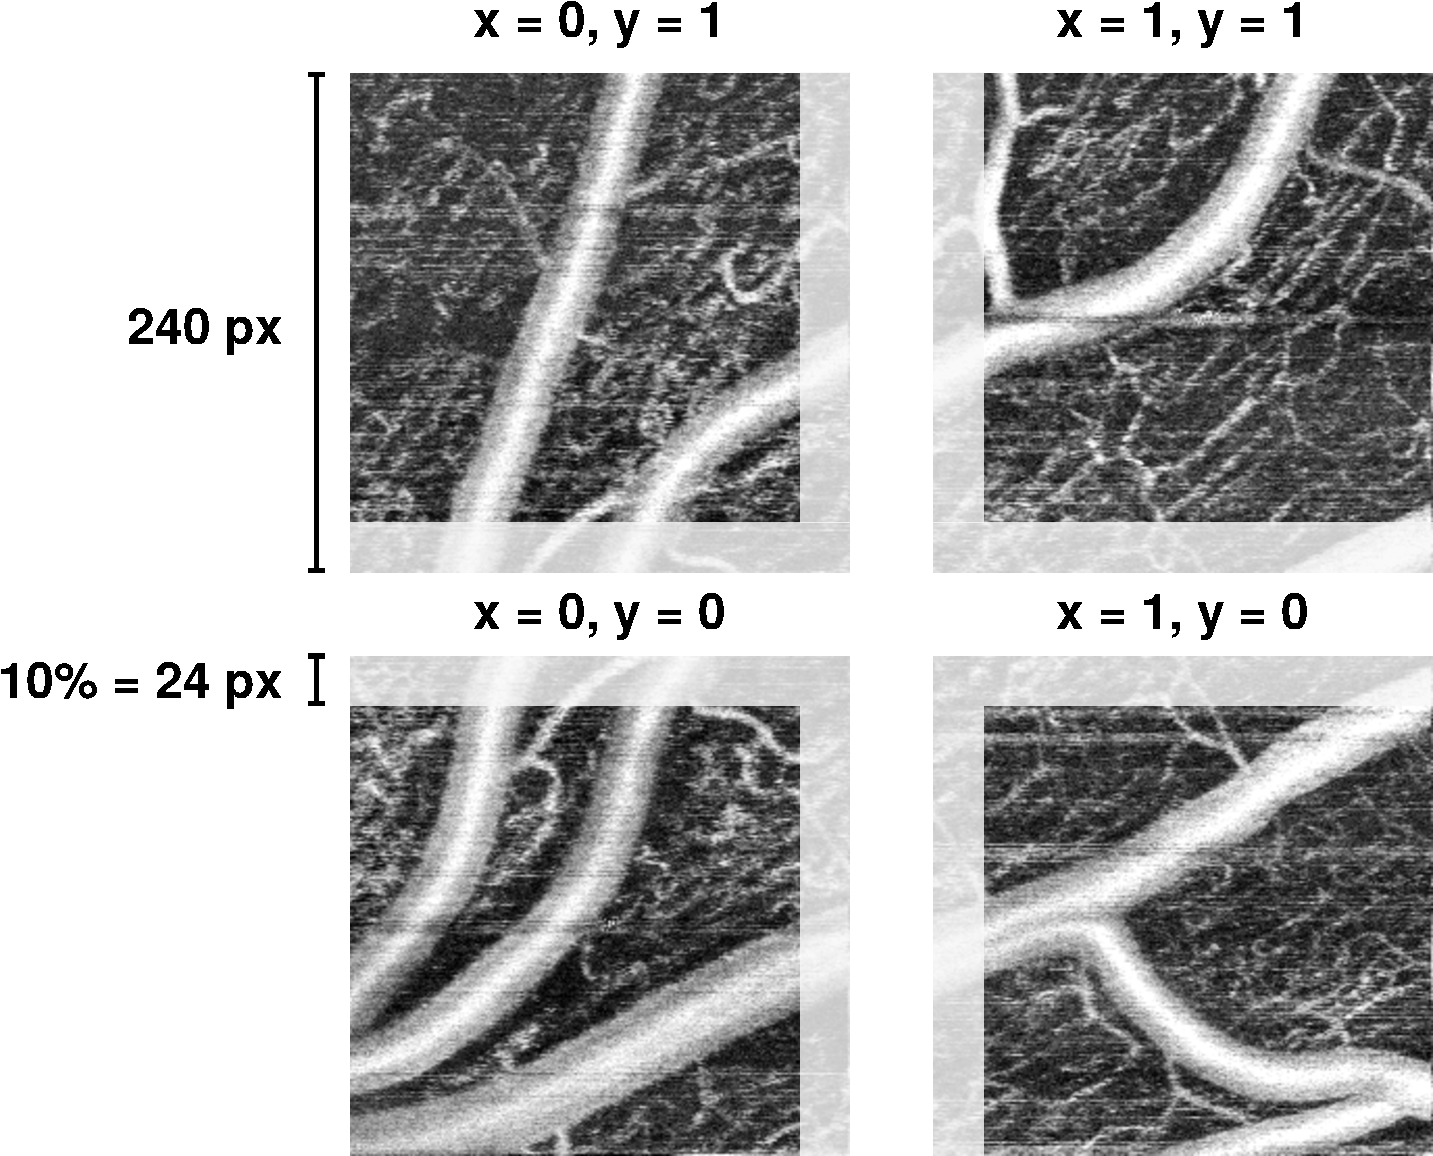
\includegraphics[width=\textwidth]{gfx/example}
  \caption{Cztery kafelki rozmieszone zgodnie z ich pozycją w docelowej mozaice. Na każdym obrazie białym przeźroczystym prostokątem zaznaczony jest oszacowany obszar nałożenia sąsiadujących kafelków.}
  \label{fig:proponowane_algorytmy:example}
\end{figure}

Informacje dostarczone wraz z kafelkami mają istotny wpływ na działanie algorytmu. Jasno podane położenie kafelek informuje algorytm, który kafelek należy dopasowywać z którym (sekcja \ref{sec:proponowane_algorytmy:filtrowanie}), a szacowany obszar nałożenia określa obszar, w którym należy ekstrahować cechy (sekcja \ref{sec:proponowane_algorytmy:sift}). Bez tych informacji stworzenie mozaiki byłoby o wiele bardziej skomplikowane.

\section{Rejestracja kafelków poprzez ekstrakcję cech SIFT}
\label{sec:proponowane_algorytmy:sift}

\subsection{Dopasowanie wyekstrahowanych cech}
\label{sec:proponowane_algorytmy:filtrowanie}

\subsection{Filtrowanie dopasowań}
\label{sec:proponowane_algorytmy:filtrowanie}

\subsubsection{Filtrowanie na podstawie wiedzy dziedzinowej}
\label{sec:proponowane_algorytmy:filtrowanie_dziedzinowe}

\subsubsection{RANSAC}
\label{sec:proponowane_algorytmy:ransac}

\section{Rejestracja kafelków poprzez wykrycie położeń naczyń krwionośnych w kafelkach}
\label{sec:proponowane_algorytmy:depth_first_search}

\section{Estymacja macierzy transformacji pomiędzy kafelkami}
\label{sec:proponowane_algorytmy:estymacja}

\section{Globalna rejestracja kafelków}
\label{sec:proponowane_algorytmy:globalna_rejestracja}

\section{Łączenie kafelków}
\label{sec:proponowane_algorytmy:laczenie_kafelkow}
